\chapter[Informações Gerais]{Informações Gerais}
\label{chap:informacoesGerais}
	
	Nesta seção serão abordados alguns tópicos introdutórios ao desenvolvimento deste relatório. Para tanto, são apresentandos membros do grupos, temas seleciondas para projeto e um mecanismo de gestão das atividades.

	\section[Integrantes do Grupo]{\emph{Integrantes do Grupo}}
	\label{sec:informacoesGerais_integrantes}

		O grupo é composto por 4 alunos. A seguir são apresentados os nomes e suas respectivas matriculas.

		\label{subsubsec:informacoesGerais_integrantes_tables}
		\begin{table}[h]
			\centering 
			\begin{tabular}{r|c}

				Nome do Integrante & Matricula \\
				
				\hline

				Augusto Samuel Modesto & 12/0111314 \\
				Beatriz Ferreira Gonçalves  & 11/0058801 \\
				Maria Luciene Felix & 12/0037742 \\
				Tiago Ribeiro de Assunção & 13/0051187 \\
				
			\end{tabular}
			\caption[Tabela de Integrantes do Grupo]{Tabela de Integrantes do Grupo.}
			\label{tab:informacoesGerais_integrantes_.tables}
		\end{table}

	\section[Tema do Projeto]{\emph{Tema do Projeto}}
	\label{sec:informacoesGerais_tema}

		Para a escolha do tema, foram analisadas diversas temáticas. Entre os temas desejados estão:

		\begin{enumerate}
			\item{\textbf{C} – Implementação de rede segura usando OpenVPN;}
			\item{\textbf{J} – Implementação de IPS/IDS para monitoramento de redes;}
			\item{\textbf{K} – Implementação de servidor de instalação de aplicações.}
		\end{enumerate}

		Para a escolha do tema utilizou-se o critério de maior média das notas (prova 1 e 2) entre os grupos envolvidos na disciplina. Neste caso, o grupo conseguiu garantir o tema \emph{J - Implementação de IPS/IDS para monitoramento de redes}.  

	\section[Ferramenta de Gestão]{\emph{Ferramenta de Gestão}}
	\label{sec:informacoesGerais_ferramenta}

		Para o controle das atividades, foi utilizado a ferramenta ZenHub. Pois, trata-se de uma ferramenta simples e ágil de gerenciamento de tarefas utilizando do método Kanban. Ela é integrada ao GitHub, onde foi possível fazer o controle de versionamentos deste relatório. A utilização de ambas as ferramentas foi essencial para controlar os registros de atividades feitas.

		O \emph{board} utilizado pode ser consultado no link a seguir:
		\begin{center}
			\href{https://github.com/modestoo/Relatorio-Redes#boards}{https://github.com/modestoo/Relatorio-Redes\#boards}
		\end{center}

		A imagem a seguir ilustra o estado final da ferramenta de gerenciamento tarefas - \textbf{ZenHub}.
		\newpage

		\begin{landscape}
			\begin{figure}[h]
				\centering
				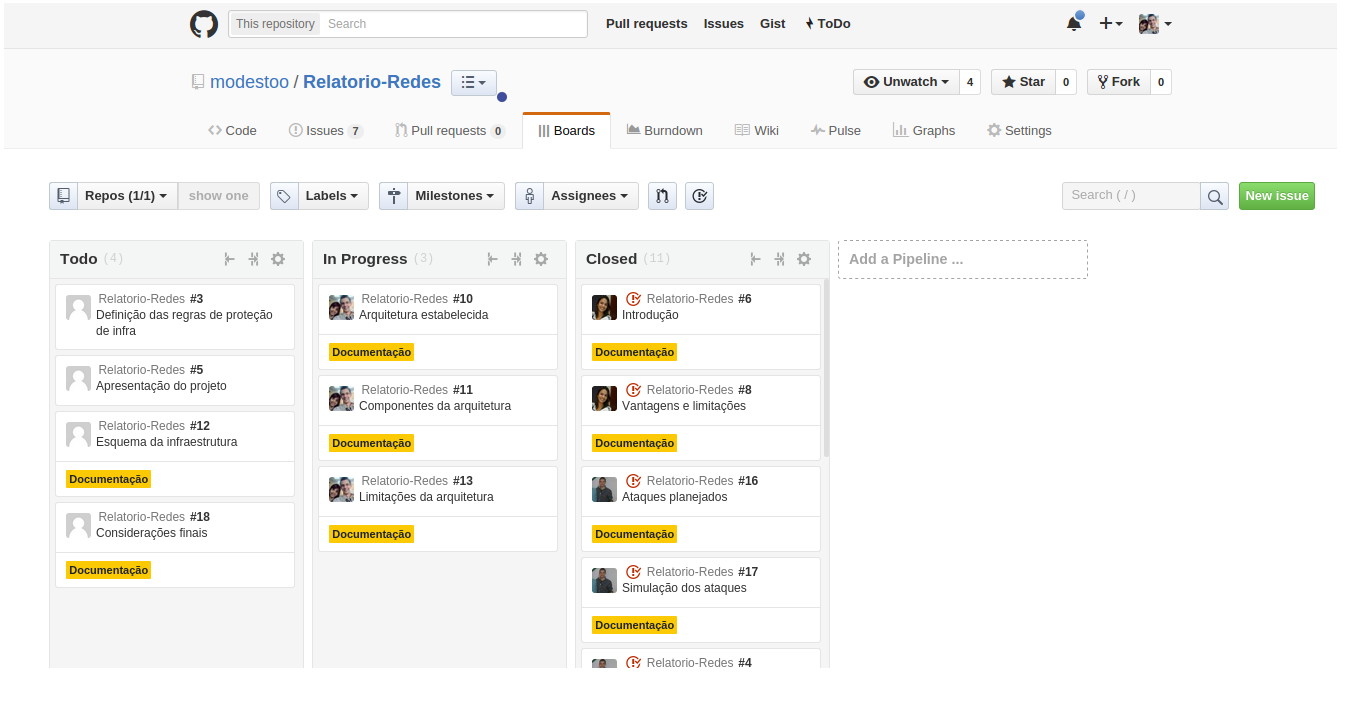
\includegraphics[scale=0.5]{zenhub}
				\caption{Ferramenta de Gestão de Atividades - ZenHub.}
				\label{fig:zenhub}
			\end{figure}
		\end{landscape}